\documentclass{article}
\usepackage{amsmath}
\usepackage{amssymb}
\usepackage{graphicx}
\usepackage{hyperref}
\usepackage[version=4]{mhchem}

\title{Example 6}
\date{}

\begin{document}
\maketitle

As shown in the figure below, in \(\triangle A B C, A D=A B . A D\) is the angle bisector of \(\angle A\). \(C M \perp A M\) at the extension of \(A D\). Show that \(A M=\frac{1}{2}(A B+A C)\).

Solution:
\begin{center}
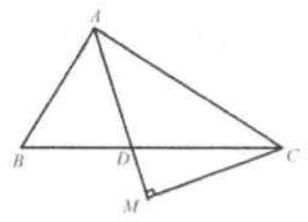
\includegraphics[width=\textwidth]{images/057(3).jpg}
\end{center}

Method 1:\\
Extend \(A M\) to \(E\) such that \(A M=M E\).\\
\(A E=2 A M=A D+D E\).\\
Now we prove that \(E C=D E\).


Since \(A D\) is the angle bisector of \(\angle A, \angle B A D=\angle C A D=\alpha\).\\
Since \(A C=C E, \angle C E A=\angle C A E=\alpha\).\\
Since \(A B=A D, \angle A B D=\angle A D B=\beta\).\\
We also know that \(\angle A D B=\angle C D E=\alpha\). (vertical angles).\\
Thus \(\angle E C D=\angle E D C=\beta\). So \(E C=D E\).\\
\(2 A M=A D+D E=A D+E C \Rightarrow A M=\frac{1}{2}(A B+A C)\).\\
\centering
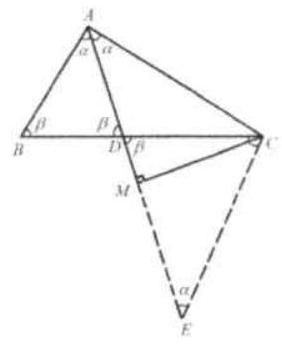
\includegraphics[width=\textwidth]{images/058(1).jpg}

Method 2:
Extend \(C M\) to \(E\) to meet the extension of \(A B\) at \(E\). So \(A E\) \(=A C\).

Draw \(M N / / E A\) to meet \(B C\) at \(N\).\\
Since \(A D\) is the angle bisector of \(\angle A, A M\) is the angle bisector of \(\angle A\). So \(\angle E A M=\angle C A M=\alpha \cdot A E=A C\)\\
\centering
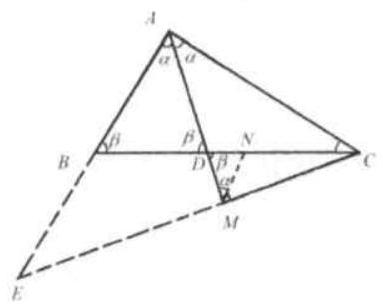
\includegraphics[width=\textwidth]{images/058.jpg}

Since \(M N / / E A, \angle B A D=\angle N M D=\alpha\).\\
Since \(A B=A D, \angle A B D=\angle A D B=\beta\).\\
We also know that \(M\) is the midpoint of \(C E . M N / / E B\), so \(M N=\frac{1}{2} B E\).\\
In \(\triangle M D N, \angle N M D=\alpha, \angle N D M=\beta\). So \(\angle M N D=\beta\).\\
Thus \(M N=D M\).\\
\(A M=A D+D M=A B+M N=A B+\frac{1}{2} B E=A B+\frac{1}{2}(A E-A B)=A B+\frac{1}{2}(A C\) \(-A B)=\frac{1}{2}(A B+A C)\).


\end{document}
